\documentclass[12pt, titlepage]{report}
\usepackage{consumer_resource_final}
\graphicspath{{./figures/}}

\begin{document}
As explained in Methods \ref{sec : methods feasibility}, before addressing the question of the stability of a system, be it dynamical or structural, it is important to study whether that system is \important{feasible}. In short we must answer the question : ``does it make sense to talk about this system? Does it even exist?''.

We will say that it makes sense to talk about a system if it is \important{feasible} (see Methods \ref{sec : methods feasibility basic concepts}). In order to be feasible, a system should respect two conditions : it must conserve biomass and its parameters must have a direct biological interpretation.

\subsection{The feasibility volume $\mathcal{V}^{G,A}_x$}
Formally we can define $\forall x \in [0,1]$ the $x$-feasibility volume $\mathcal{V}^{G,A}_x \subset \mathcal{M}$ of the consumption network coupled with the syntrophy network $(G, A) \in \mathcal{B}_{N_S \times N_R} \times  \mathcal{B}_{N_R \times N_S}$ (see Methods \ref{sec : methods feasibility volume}). Every metaparameter set $m \in \mathcal{M}$ contained in the $x$-feasibility volume $\mathcal{V}^{G,A}_x$ will give rise to a percentage $x$ of feasible systems. A first order approximation of the fully feasible volume $\mathcal{V}^{G,A}_1$ is given by Eq.\eqref{eq : fully feasible volume}.
% , which we recall here:
% \begin{equation}
% \max_i\left\{\frac{\deg(A,i)}{\deg(G,i)}\right\} \alpha_0
% \lessapprox \min(1-\sigma_0, \sigma_0) \gamma_0 R_0
% \lessapprox
% \min \left(1-\sigma_0, \sigma_0 \right) \min_\nu \left\{ \frac{l_0}{\deg(G,\nu) S_0} + \frac{\deg(A,\nu)}{\deg(G,\nu)}\alpha_0\right\}.
% \end{equation}
In the absence of syntrophy $\alpha_0=0$, it becomes :
\begin{equation}
\gamma_0 R_0 \lessapprox \frac{l_0}{\max_\nu\{\deg(G,\nu)\}S_0}. \label{eq : fully feasible volume no syntrophy}
\end{equation}
This relation is interesting in many ways. First of all it tells us that at fixed consumption rate $\gamma_0$ and resource equilibrium abundance $R_0$, feasibility increases when :
\begin{itemize}
\item the external resource input rate increases. This result was somewhat expected : if you give more food to a goldfish you expect it to thrive more.
\item the consumer equilibrium abundance $S_0$ increases. What this means is that if you want to maintain the same consumption interaction but get a higher abundance of resources at equilibrium, you must at the same time decrease the consumers equilibrium abundance.
\item the largest column-degree of the consumption matrix decreases. The degree of a given column $\nu$ of the consumption matrix tells you how many species eat from resource $\nu$. This encourages communities of specialists, where each consumer eats from its own and no other resource.
\end{itemize}
Overall we see that feasibility increases when the \important{consumption flow} $\simeq \gamma_0 S_0 \deg(G,\nu) $ is low $\forall \nu$.
Eq.\eqref{eq : fully feasible volume no syntrophy} can be confronted to simulations. Figure \ref{fig : typical feasibility region} shows the proportion of feasible systems without syntrophy $\mathcal{F}(\gamma_0, S_0, \alpha_0=0, G)$ and $R_0=l_0=1$, $\sigma_0=0.25$ (see Methods \ref{sec : methods feasibility volume}), for two matrices $G_1$ and $G_2$ of our set. $G_1$ has connectance $\kappa_1=0.17$ and nestedness $\eta_1=0.2$, $G_2$ is more connected and more nested : $\kappa_2=0.37$ and $\eta_2=0.4$.

We observe a very sharp transition from a fully feasible to a fully unfeasible regime. Theoretically, this sharp transition happens when both sides of the inequality \eqref{eq : fully feasible volume no syntrophy} are equal, \ie at $\gamma_0 R_0 = l_0/\max_\nu\{\deg(G,\nu)\}S_0$.
 Numerically we fit the points which are at ``the boundary'' of the common feasible volume, \ie points where $0.4 \leq \mathcal{F}(\gamma_0, S_0, G) \leq 0.6$.

 For $G_1$, the theoretical expectation is $S_0 = 0.125/ \gamma_0$ and a fit on the numerical results gives $S_0=(\num[scientific-notation=false]{0.124}\pm\num{7e-8})/ \gamma_0 - (\num{6.8e-4}\pm\num{3e-7})$ so the theoretical relation is already very good.
For $G_2$, we expect $S_0 = 0.077 /\gamma_0$. A fit gives $S_0=(\num[scientific-notation=false]{0.075}\pm\num{2e-8})/\gamma_0 +(\num{3.6e-4}\pm\num{1e-7})$. Again, the theoretical value is very close to the measured value.
\begin{figure}[h!]
\centering
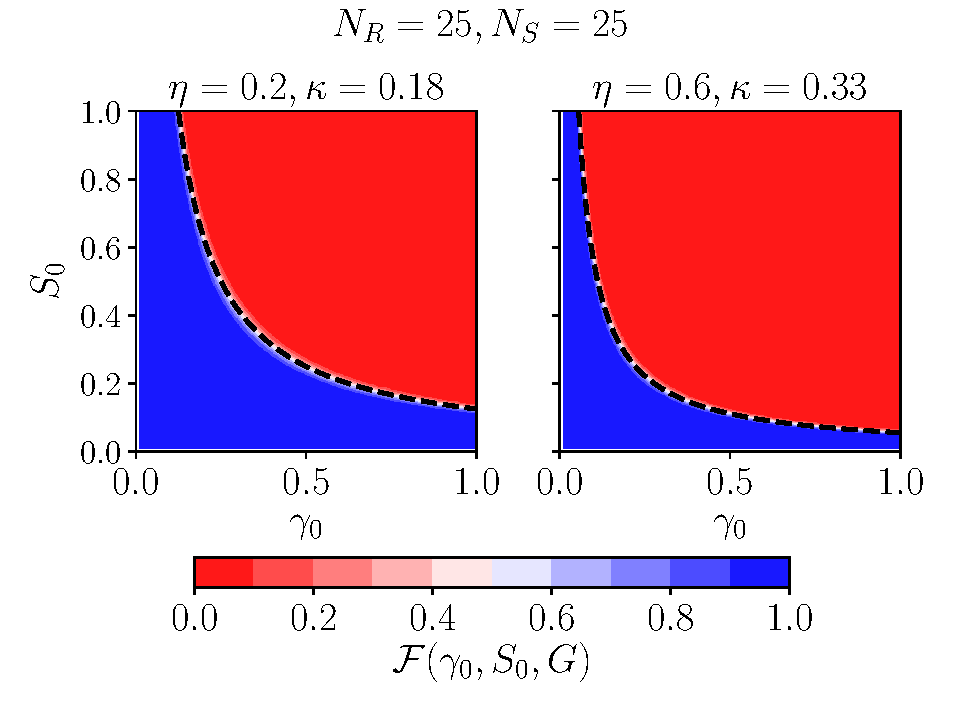
\includegraphics[width=0.7\linewidth]{Results/typical_feasibility_volume}
\caption{Plot of the feasability region. The color curve indicicates the feasibility function $\mathcal{F}(\gamma_0, S_0, \alpha_0=0, G)$ for $G_1$ (left) and $G_2$ (right). We observe a steep descent which marks a very clear transition from a totally feasible regime to a totally unfeasible regime, which allows us to precisely get the boundary of $\mathcal{V}^{G}_1$. The dashed lines indicate the theoretical predictions, which for both $G_1$ and $G_2$ are accurate to the order of $0.1 \%$.}
\label{fig : typical feasibility region}
\end{figure}

The numerical estimate does not always match that well the theoretical value. Fig.\ref{fig : deviation away from theory feasibility} shows the relative error $\Delta_G = 1 -$ (theoretical value)/(numerical estimate). We see that in general the theoretical expectation tends to overestimate the fully feasible region. This is probably due to the noise (\ie the deviations away from the metaparameters) in the actual systems and the structure of the $G$ matrix. Indeed Fig.\ref{fig : deviation away from theory feasibility} shows that the lower the nestedness and connectance of $G$, the worse the theoretical estimate. In the future a better approximation can surely be found taking into account the variance of the metaparameters and the nestedness of $G$.
\begin{figure}[h!]
	\captionsetup[subfigure]{captionskip = -165pt, margin = 45pt}
\subfloat[\label{fig : deviation away from theory feasibility fixed nestedness}]{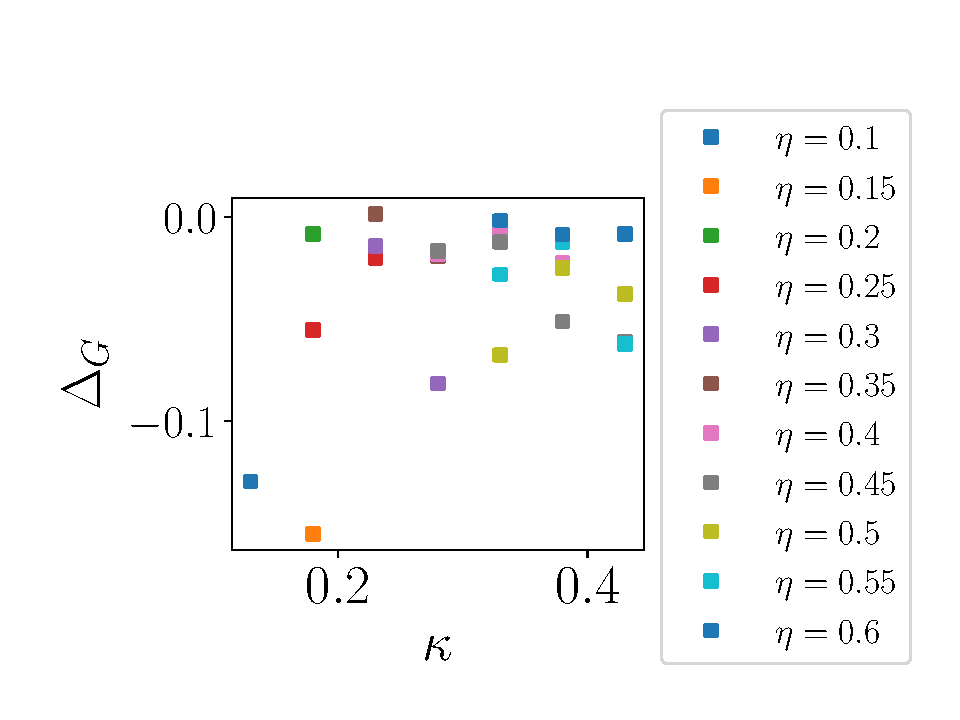
\includegraphics[width=0.49\linewidth]{Results/feasibility_away_from_theory_fixed_nestedness}}
\captionsetup[subfigure]{captionskip = -175pt, margin = 45pt}
\subfloat[\label{fig : deviation away from theory feasibility fixed connectance}]{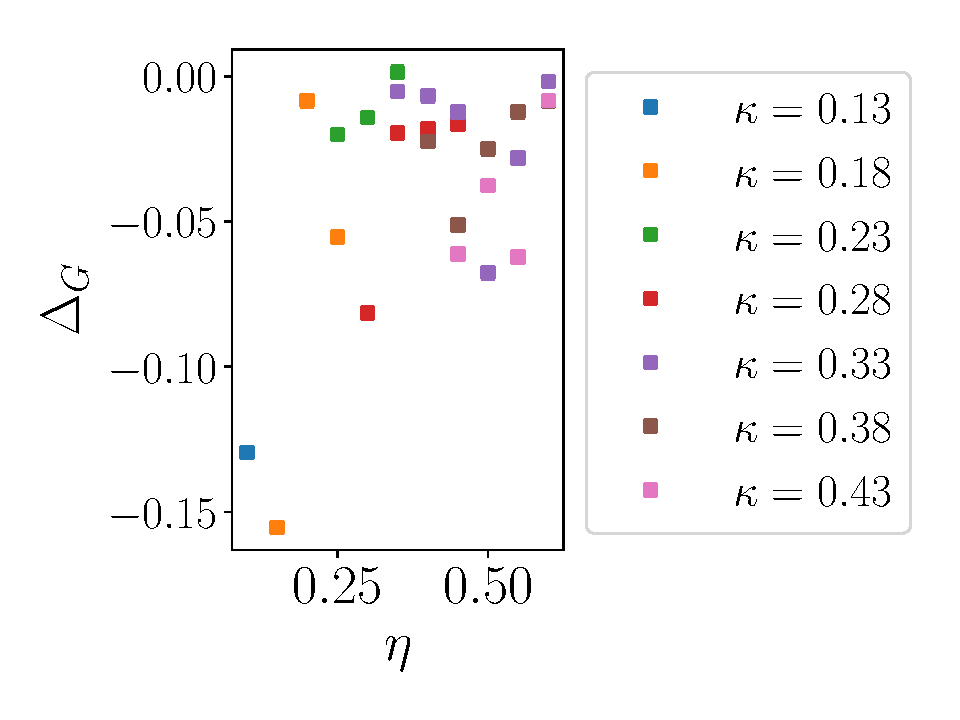
\includegraphics[width=0.49\linewidth]{Results/feasibility_away_from_theory_fixed_connectance}}
\caption{Relative error in the determination of the boundary of $\mathcal{V}^{G,0}_1$ (a) varying connectance at fixed nestedness and (b) varying nestedness at fixed connectance. The theoretical prediction tends to overestimate the measured value. The larger the nestedness and connectance, the better the estimate.}\label{fig : deviation away from theory feasibility}
\end{figure}

We can similarly measure the common fully feasible volume $\mathcal{V^*}$, which according to Eq.\eqref{eq : fully feasible volume no syntrophy} is inversely proportional to the largest maximal row degree of the matrix set. For the set we considered, this yields in theory : $S_0 = 0.053 \gamma_0$. A fit on the points at the edge yields the critical boundary $S_0 = (0.043 \pm 10^{-8})/\gamma_0 - (4.6 \times 10^{-3} \pm 3 \times 10^{-8})$. The theoretical prediction is not as good as before with an error of $\sim 20 \%$. The discrepancy is probably due to the fact that numerically we determine the common feasibility volume by counting the points for which $\mathcal{F}(\gamma_0, S_0, G)=1 \ \forall G \in S_G$.
while the theoretical value matches better a fit of the points $0.4 \leq \mathcal{F} \leq 0.6$ \textbf{make this more understandable}.
\begin{figure}[h!]
\centering
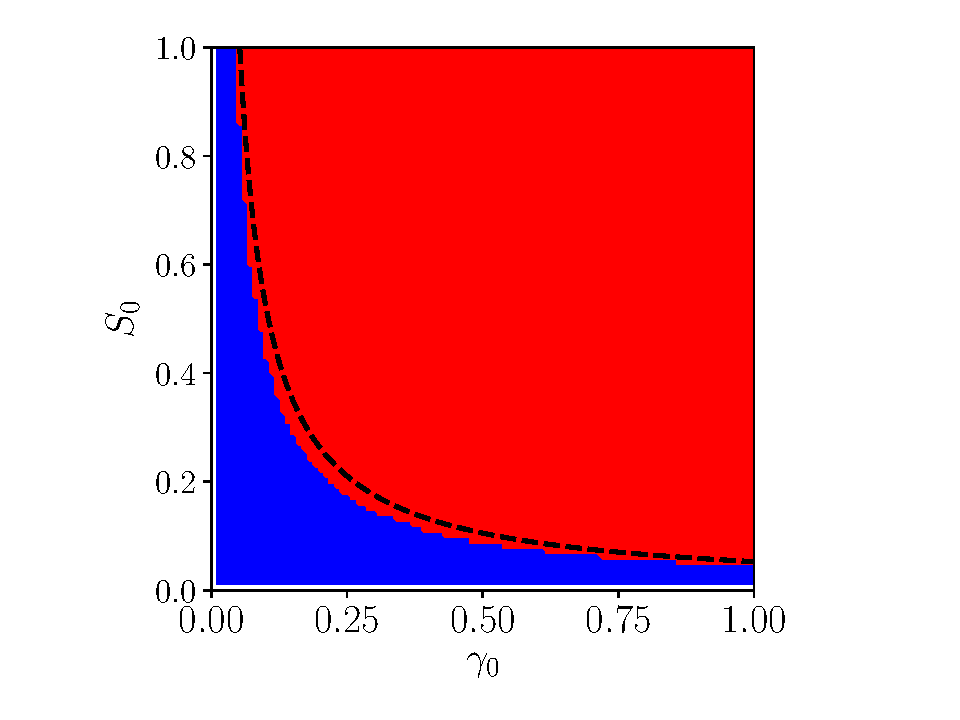
\includegraphics[width=0.7\linewidth]{Results/common_feasibility_volume}
\caption{Plot of the common feasability region. The blue area indicates the common feasibility volume, computed numerically, while the dashed line shows the analytical prediction. Although the match is not as good as before, the relative error is only of the order of $20 \%$. The red part is the area where not all matrices are fully feasible. From now on, it will not be considered anymore.}
\label{fig : common feasible volume}
\end{figure}

\subsection{Evolution of the fully feasible volume with syntrophy}

\begin{figure}[h]
\hspace{-0.1\linewidth}
\subfloat{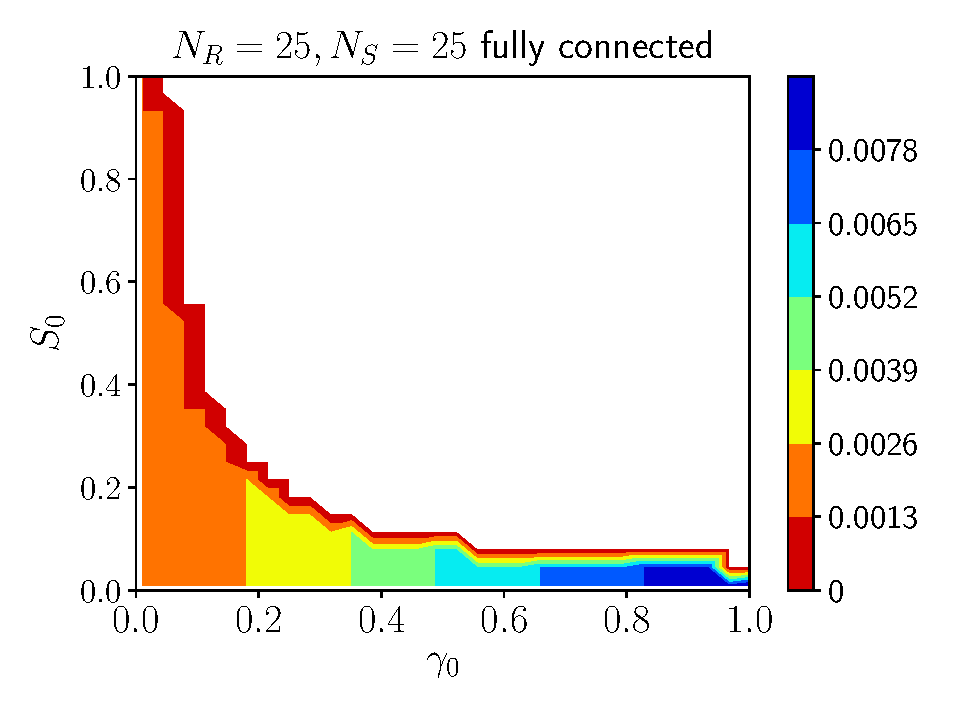
\includegraphics[width=0.6\linewidth]{Results/common_feasibility_volume_varying_syntrophy_random_structure}}
\subfloat{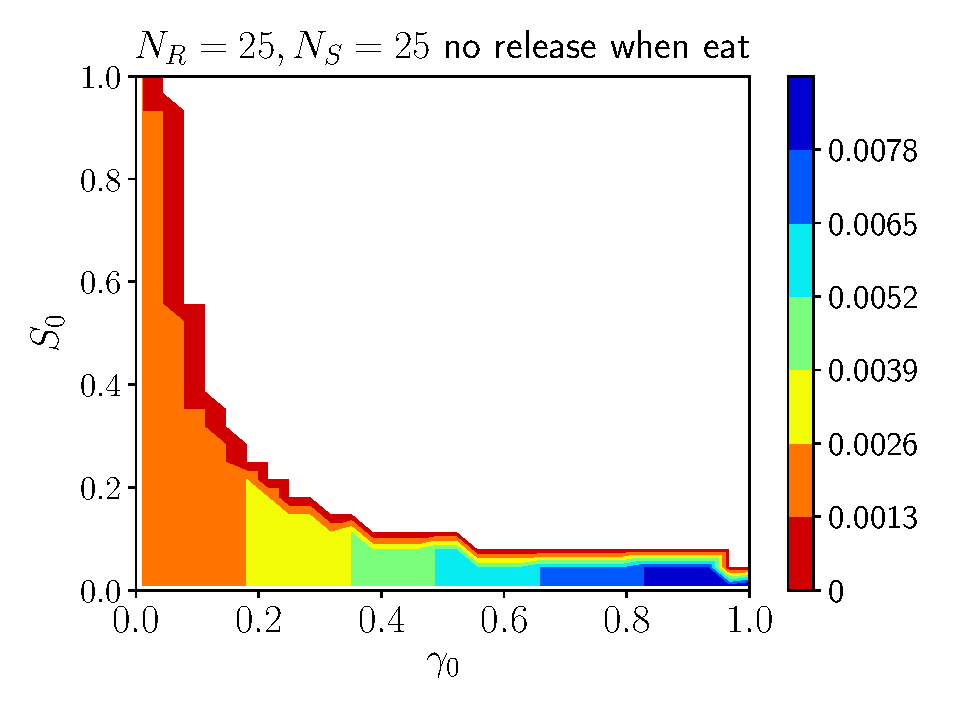
\includegraphics[width=0.6\linewidth]{Results/common_feasibility_volume_varying_syntrophy_no_release_when_eat}}
\begin{center}
\subfloat{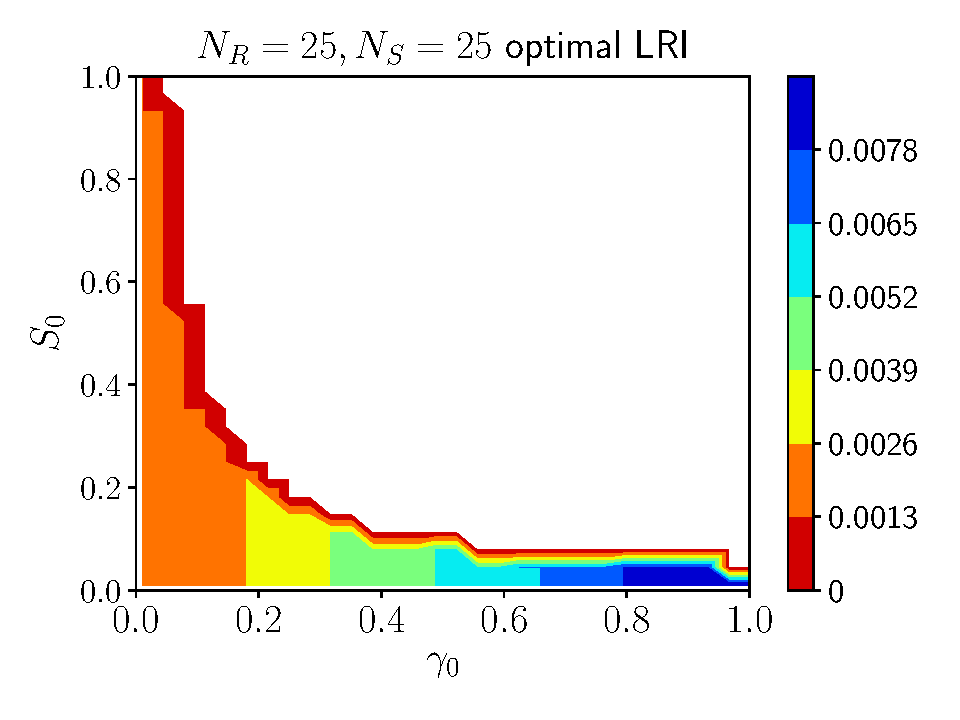
\includegraphics[width=0.6\linewidth]{figures/Results/common_feasibility_volume_varying_syntrophy_optimal_matrix}}
\end{center}
\caption{Evolution of the fully feasible volume as syntrophy grows. Note that even though it is not very clear on the figure $\mathcal{V}^*(\alpha_0^+) \subset \mathcal{V}^*(\alpha_0^-) \ \forall \alpha_0^+ > \alpha_0^-$, \ie the common fully feasible region of higher syntrophy is included in the one of lower syntrophy.}
\end{figure}

\end{document}
